\section{Test period}
To evaluate the proposed solution against the current control system, both are simulated with the same historical data for both consumption and weather for a range of days. It is important to test the control system performance on a period not included in the design of the control system. Hence, the week from \textbf{2023-12-24 00:00} to \textbf{2024-01-01 00:00} was chosen because it \textbf{contains no data used in the control system design}. Furthermore, as seen in figure \ref{fig:tot_con_chiwoza_20231201-20240115} the daily consumption is relatively normal, avoiding the days before December 24th 2023 used in the development of the models, and the large abnormal drop in measured consumption on January 2nd 2024. The maximum theoretical production, based on weather measurements and the model in equation \ref{eq:pv_prod_physical_model} suggest somewhat varying conditions for production as shown in figure \ref{fig:prod_theoretic_chiwoza_20231207-20240115}, yielding an interesting case for the control system.

\begin{figure}[h]
    \centering
    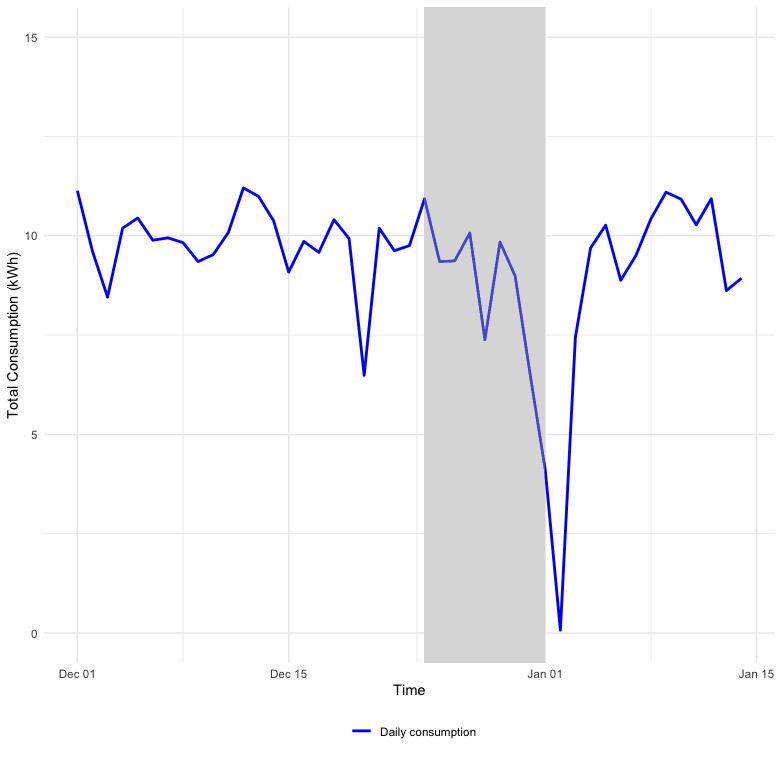
\includegraphics[width=\textwidth]{Figures/09Results/tot_con_chiwoza_20231201-20240115.png}
    \caption[Total daily consumption Chiwoza 20231201-20240115]{Total daily consumption Chiwoza from December 1st 2023 to January 15th 2024. The shaded area represents the dates from December 24th 2023 to January 1st 2024 used as the testing period for the control system.}
    \label{fig:tot_con_chiwoza_20231201-20240115}
\end{figure}

\begin{figure}[h]
    \centering
    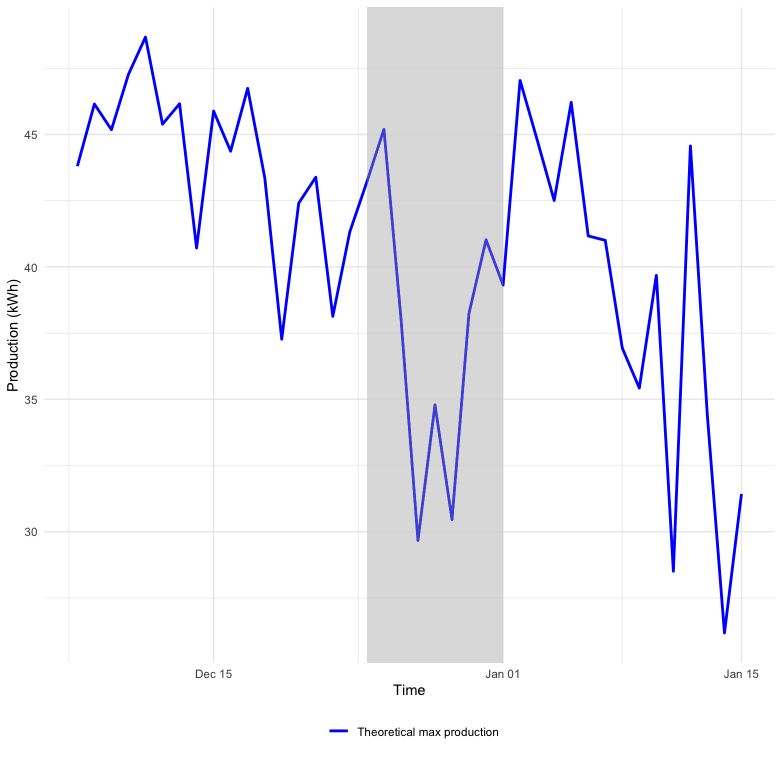
\includegraphics[width=\textwidth]{Figures/09Results/prod_theoretic_chiwoza_20231207-20240115.png}
    \caption[Theoretical max production Chiwoza 20231207-2024015]{Maximum theoretical production based at Chiwoza from December 7th 2023 to January 15th 2024 based on the model in equation \ref{eq:pv_prod_physical_model}. The shaded area represents the dates from December 24th 2023 to January 1st 2024 used as the testing period for the control system.}
    \label{fig:prod_theoretic_chiwoza_20231207-20240115}
\end{figure}

\section{Simulation candidates}
Results from 4 different simulations using currently installed equipment are included. All simulating with the same data and conditions. The candidates are:
\begin{itemize}
    \item \textbf{Current control system}
    \item \textbf{Proposed control system with tuning 1} - Tuned for critical load reliability.
    \item \textbf{Proposed control system with tuning 2} - Tuned for battery health
    \item \textbf{Proposed control system with tuning 2 using perfect demand forecasts} - Unrealistic case of the control system knowing all demand perfectly in advance.
\end{itemize}

Over the same data, the current control system and proposed control system with tuning 2 are also simulated with three different levels of installed battery capacity.

\section{Simulation results}
\subsection{Power Flow}

The power flow shows the high-level flow of power in the system. The consumption and production are plotted as a time-series against the primary y-axis, while the State of charge is plotted against the secondary y-axis. A higher production than consumption indicates the charging of the battery, while a higher consumption than production indicates battery discharge. The plots for the current control system, tuning 1 and tuning 2 is found in figure \ref{fig:pf_231224-240101_CS_soiling26}, \ref{fig:pf_231224-240101_tuning1_soiling26} and \ref{fig:pf_231224-240101_tuning2_soiling26} respectively. 

\begin{figure}[h]
    \centering
    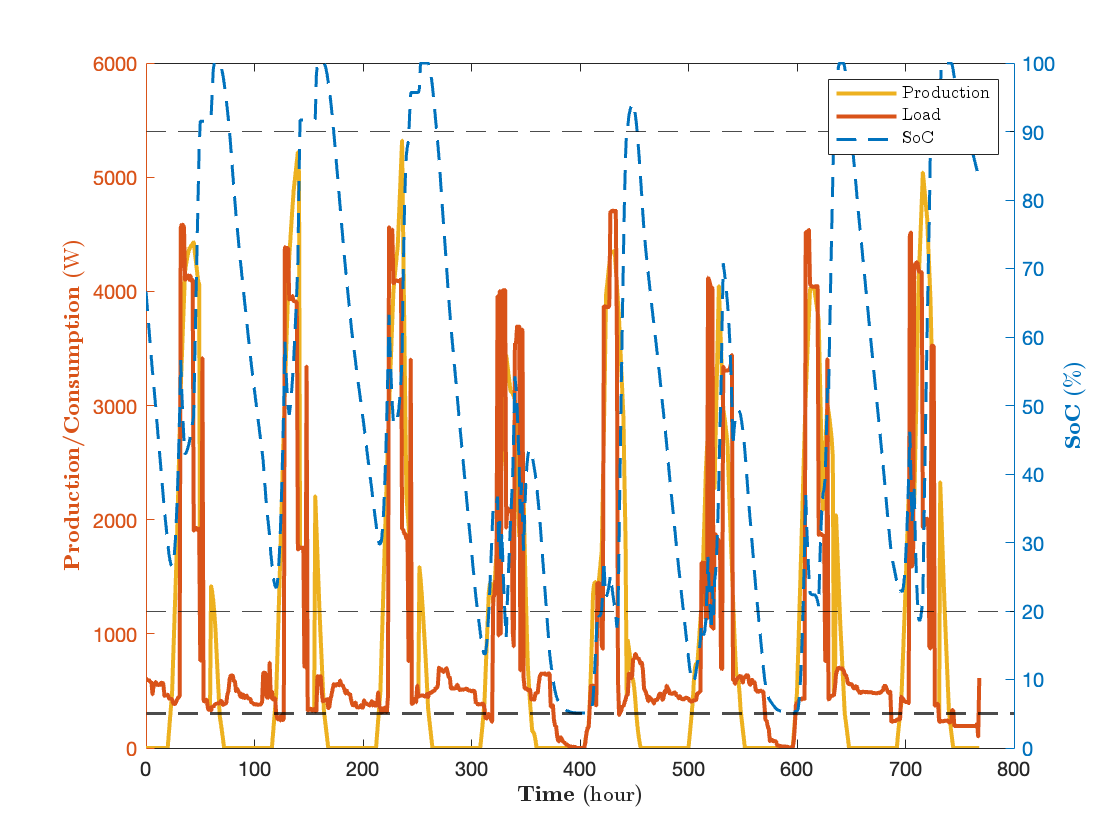
\includegraphics[width=\textwidth]{Figures/09Results/pf_231224-240101_CS_soiling26.png}
    \caption[Power flow current control system]{Production, consumption and SOC for the current control system. The horizontal red stapled lines are thresholds for the battery. }
    \label{fig:pf_231224-240101_CS_soiling26}
\end{figure}

\begin{figure}[h]
    \centering
    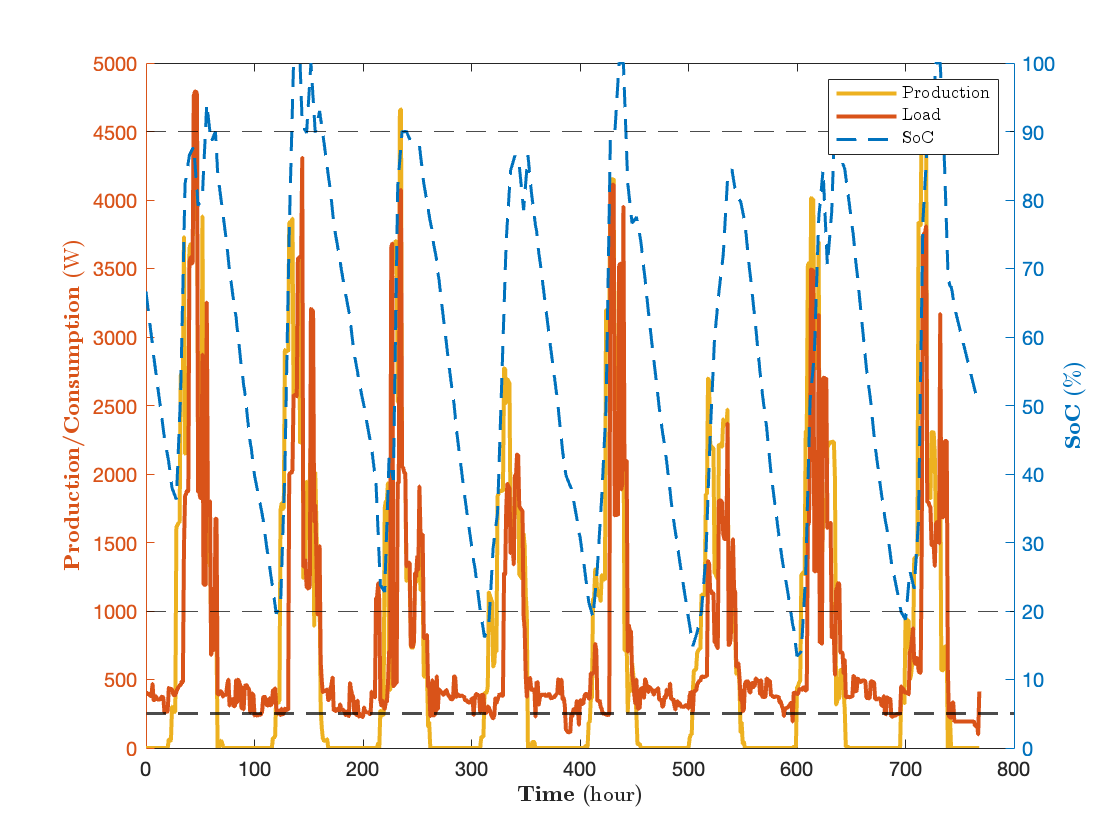
\includegraphics[width=\textwidth]{Figures/09Results/pf_231224-240101_tuning1_soiling26.png}
    \caption[Power flow proposed control system 1]{Production, consumption and SOC for the proposed control system with tuning 1. The horizontal red stapled lines are thresholds for the battery. }
    \label{fig:pf_231224-240101_tuning1_soiling26}
\end{figure}

\begin{figure}[h]
    \centering
    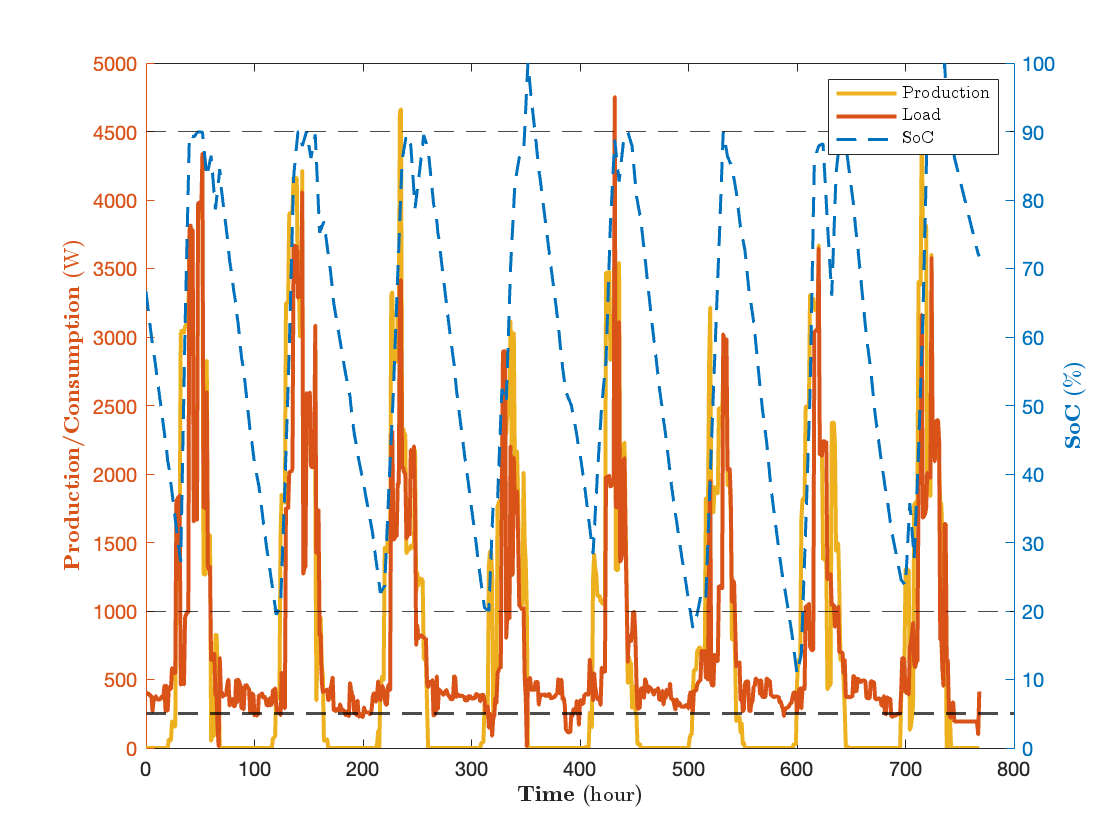
\includegraphics[width=\textwidth]{Figures/09Results/pf_231224-240101_tuning2_soiling26.png}
    \caption[Power flow proposed control system 2]{Production, consumption and SOC for the proposed control system with tuning 2. The horizontal red stapled lines are thresholds for the battery. }
    \label{fig:pf_231224-240101_tuning2_soiling26}
\end{figure}

\begin{figure}[h]
    \centering
    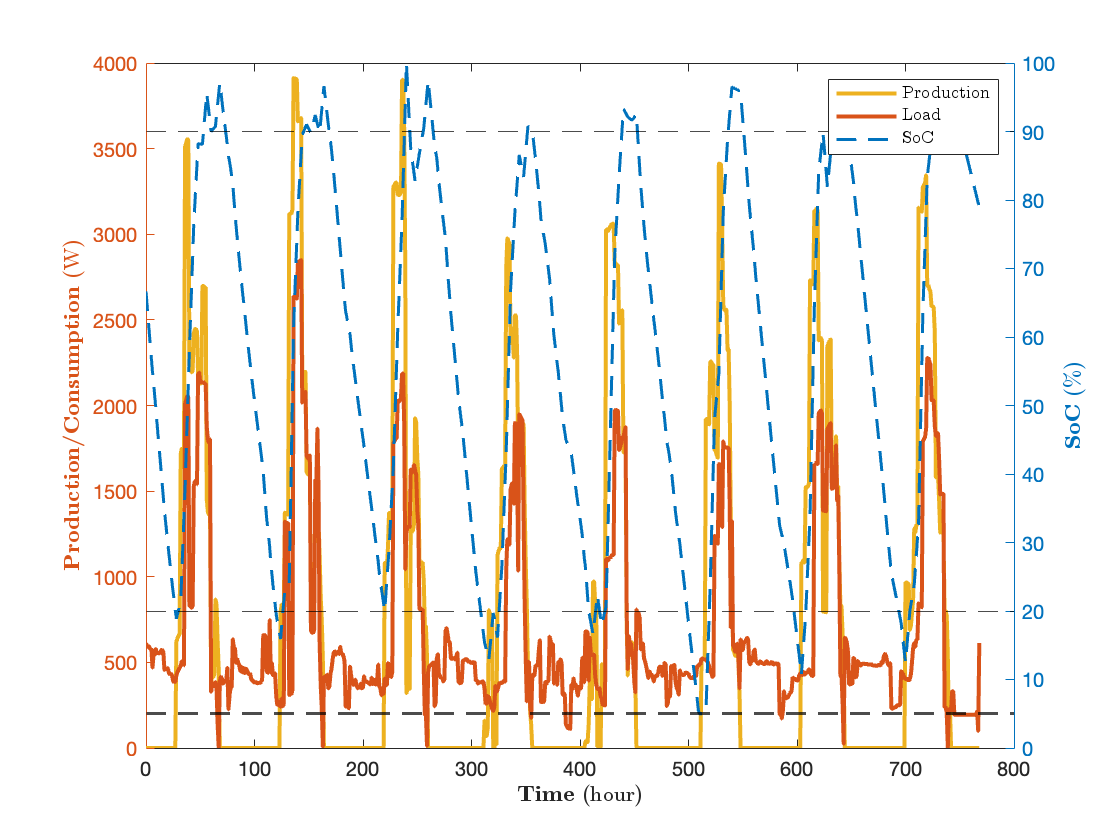
\includegraphics[width=\textwidth]{Figures/09Results/pf_231224-240101_tuning2_perfectR.png}
    \caption[Power flow proposed control system 2 perfect demand estimation]{Production, consumption and SOC for the proposed control system with tuning 2 using perfect demand estimation. The horizontal red stapled lines are thresholds for the battery. }
    \label{fig:pf_231224-240101_tuning2_perfectR}
\end{figure}

\subsection{Unmet Demand}

Unmet demand is when a load has requested a certain amount of power, but has not been supplied it. In figure \ref{fig:error_231224-240101_CS_soiling26}, \ref{fig:error_231224-240101_tuning1_soiling26} and \ref{fig:error_231224-240101_tuning2_soiling26} the unmet demand is plotted with its magnitude and time of occurrence for the current control system, tuning 1 and tuning 2 respectively. In figure \ref{fig:error_perc_231224-240101_CS_soiling26}, \ref{fig:error_perc_231224-240101_tuning1_soiling26} and \ref{fig:error_perc_231224-240101_tuning2_soiling26} the amount of times a load has its demand unmet as a ratio to the total length of the simulation is graphed.

\begin{figure}[h]
    \centering
    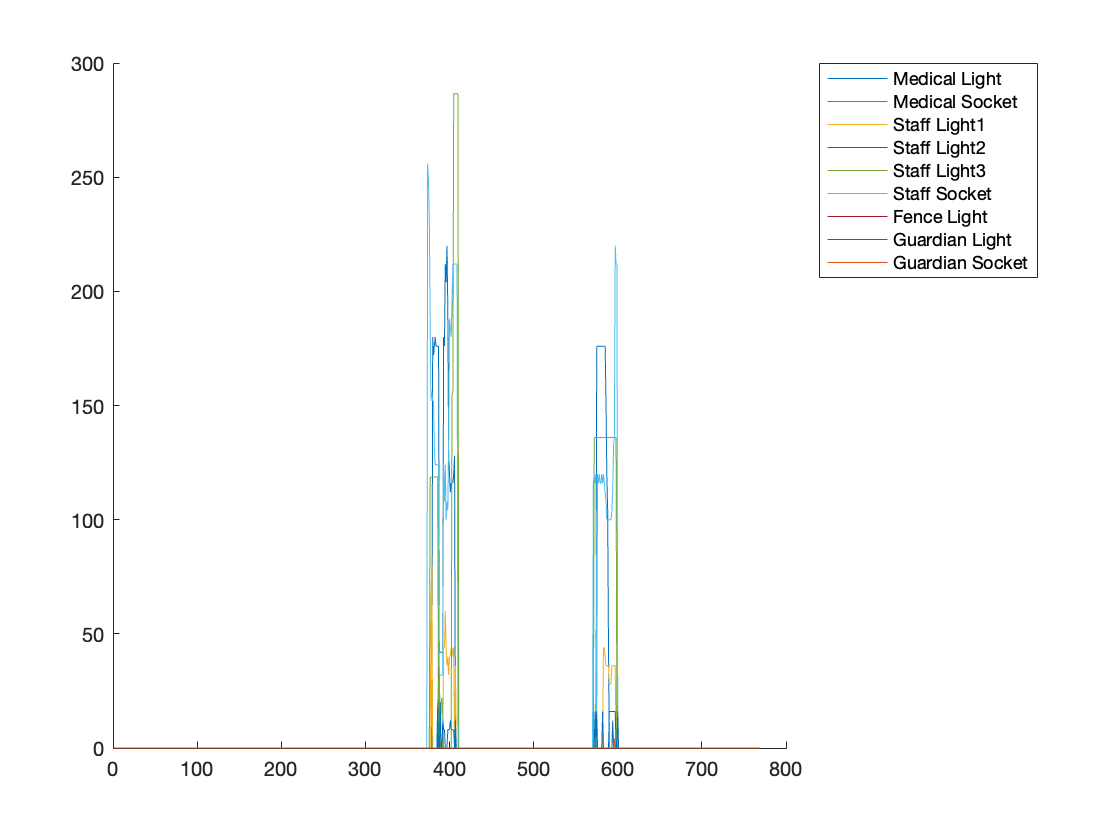
\includegraphics[width=\textwidth]{Figures/09Results/error_231224-240101_CS_soiling26.png}
    \caption[Unmet demand current control system]{Unmet demand across the period for the current control system. }
    \label{fig:error_231224-240101_CS_soiling26}
\end{figure}

\begin{figure}[h]
    \centering
    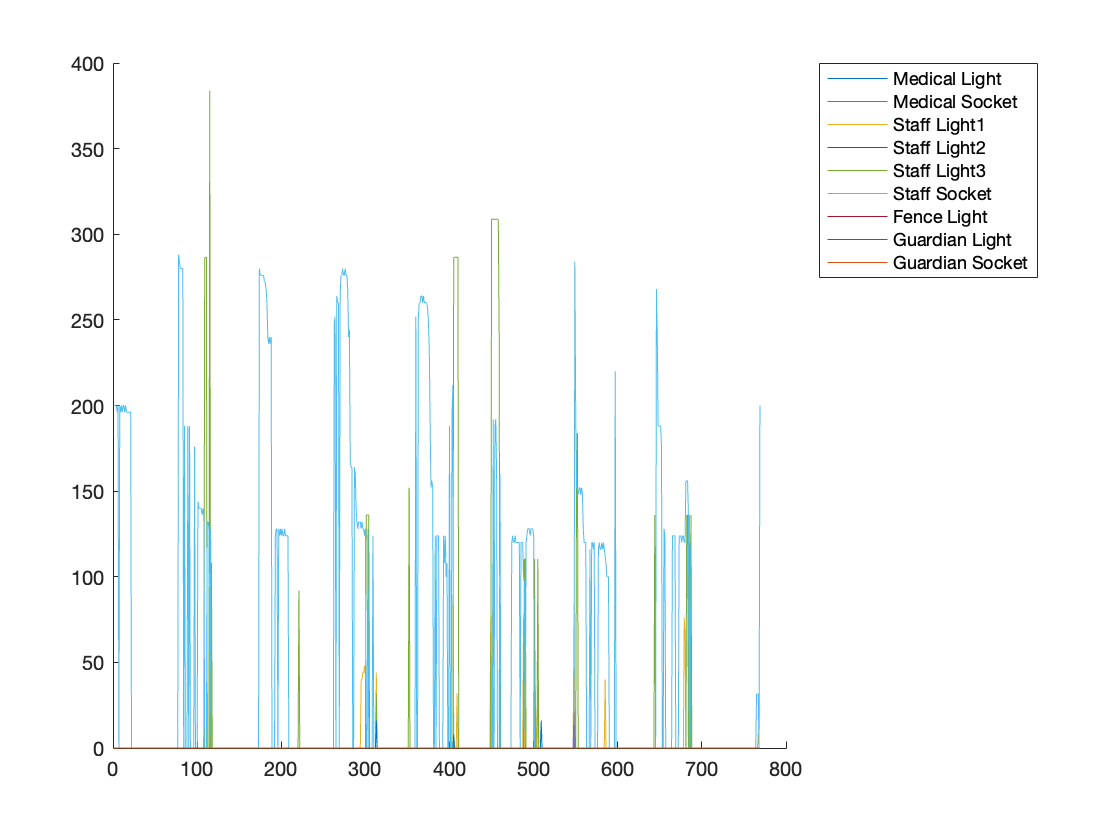
\includegraphics[width=\textwidth]{Figures/09Results/error_231224-240101_tuning1_soiling26.png}
    \caption[Unmet demand proposed control system 1]{Unmet demand across the period for the proposed control system with tuning 1. }
    \label{fig:error_231224-240101_tuning1_soiling26}
\end{figure}

\begin{figure}[h]
    \centering
    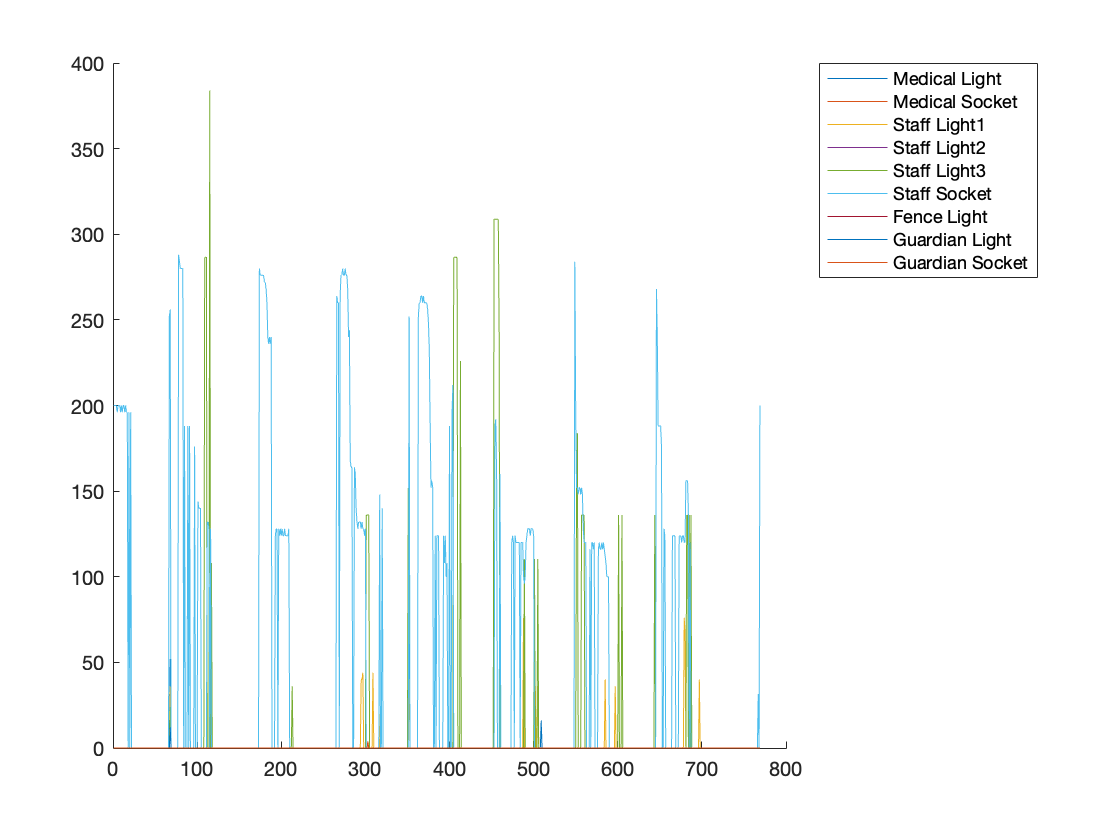
\includegraphics[width=\textwidth]{Figures/09Results/error_231224-240101_tuning2_soiling26.png}
    \caption[Unmet demand proposed control system 2]{Unmet demand across the period for the proposed control system with tuning 2. }
    \label{fig:error_231224-240101_tuning2_soiling26}
\end{figure}

\begin{figure}[h]
    \centering
    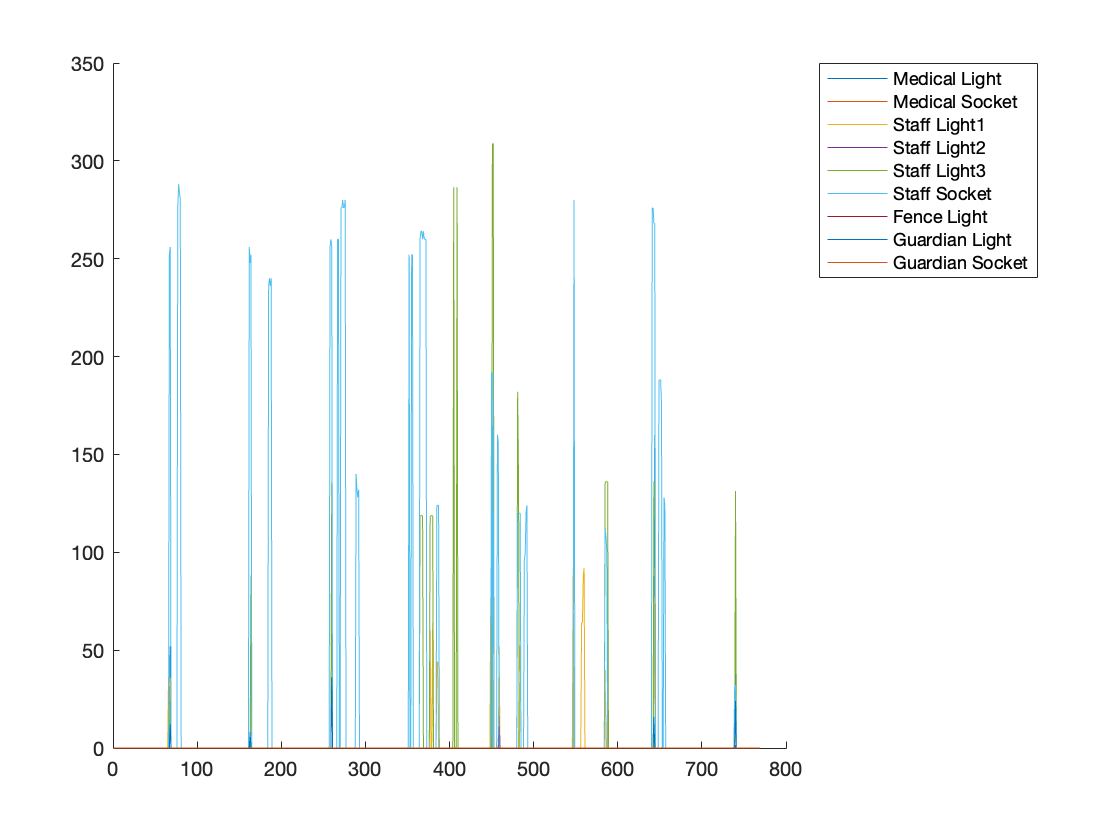
\includegraphics[width=\textwidth]{Figures/09Results/error_231224-240101_tuning2_perfectR.png}
    \caption[Unmet demand proposed control system 2 perfect R]{Unmet demand across the period for the proposed control system with tuning 2 using perfect demand estimation. }
    \label{fig:error_231224-240101_tuning2_perfectR}
\end{figure}

\begin{figure}[h]
    \centering
    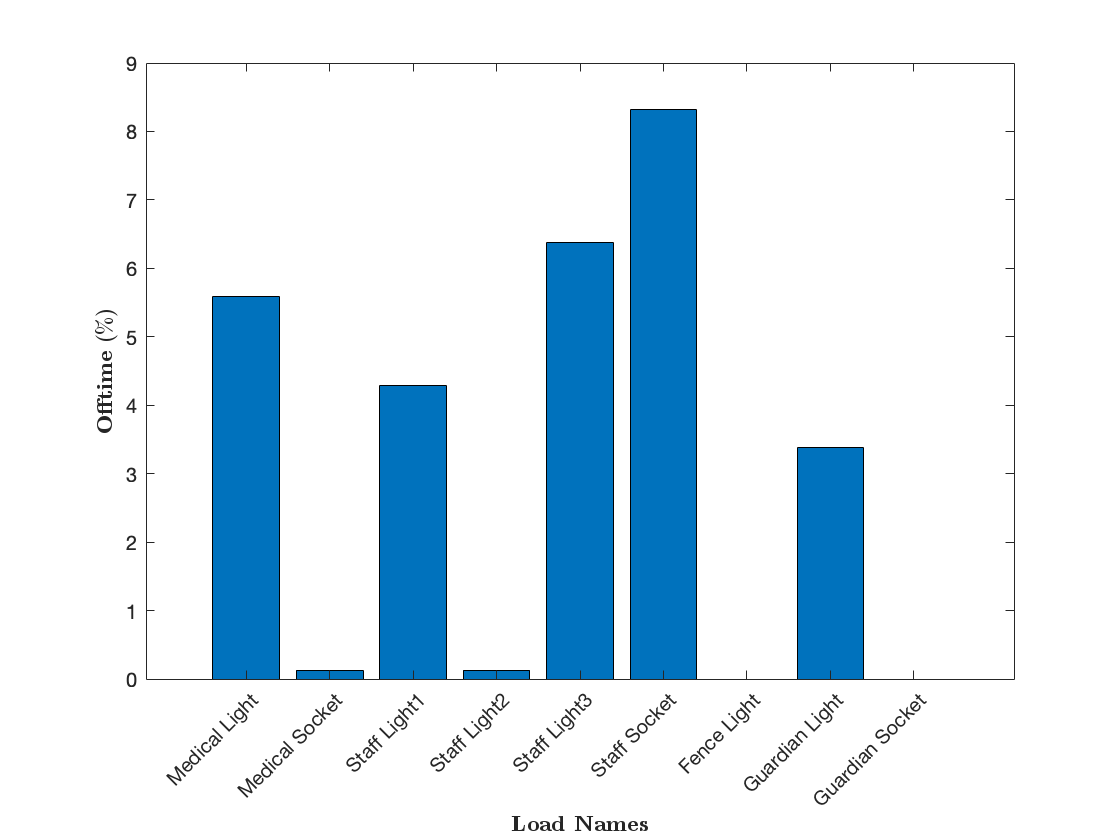
\includegraphics[width=\textwidth]{Figures/09Results/error_perc_231224-240101_CS_soiling26.png}
    \caption[Unmet demand portion current control system]{Number of times demand was unmet as a percentage of the whole period for the current control system. }
    \label{fig:error_perc_231224-240101_CS_soiling26}
\end{figure}

\begin{figure}[h]
    \centering
    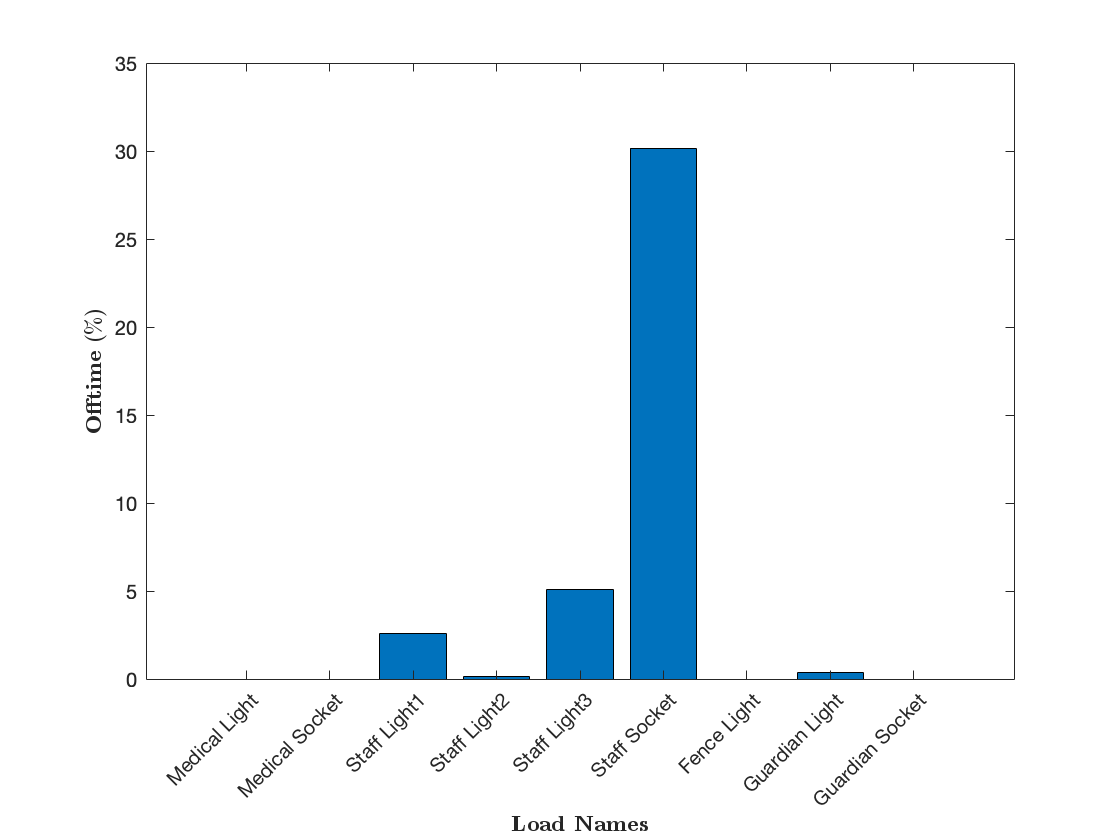
\includegraphics[width=\textwidth]{Figures/09Results/error_perc_231224-240101_tuning1_soiling26.png}
    \caption[Unmet demand portion proposed control system 1]{Number of times demand was unmet as a percentage of the whole period for the proposed control system with tuning 1. }
    \label{fig:error_perc_231224-240101_tuning1_soiling26}
\end{figure}

\begin{figure}[h]
    \centering
    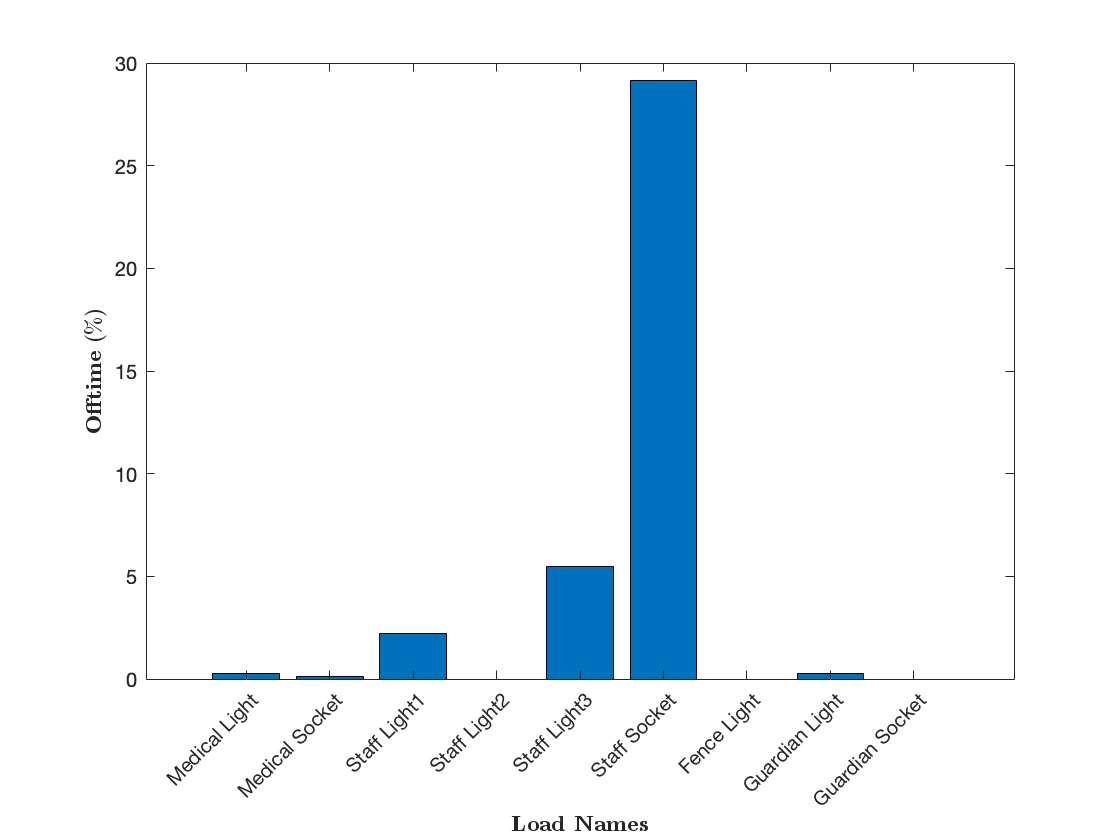
\includegraphics[width=\textwidth]{Figures/09Results/error_perc_231224-240101_tuning2_soiling26.png}
    \caption[Unmet demand portion proposed control system 2]{Number of times demand was unmet as a percentage of the whole period for the proposed control system with tuning 2. }
    \label{fig:error_perc_231224-240101_tuning2_soiling26}
\end{figure}

\begin{figure}[h]
    \centering
    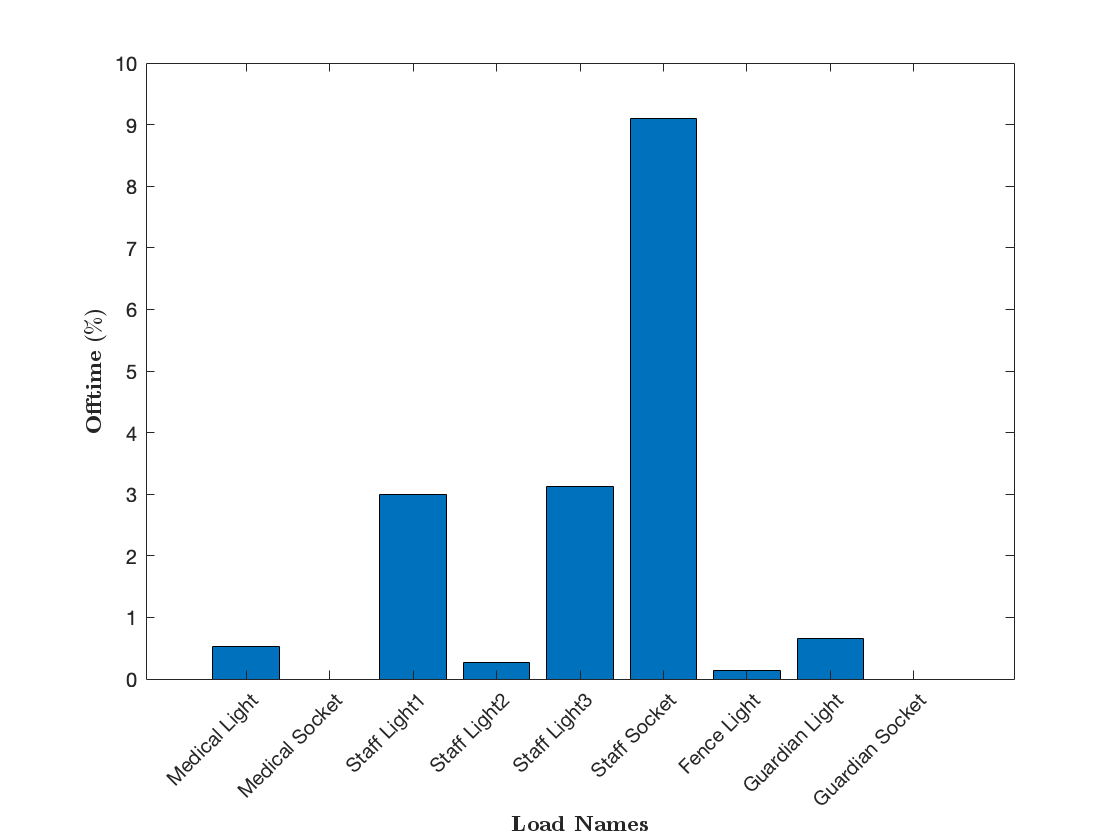
\includegraphics[width=\textwidth]{Figures/09Results/error_perc_231224-240101_tuning2_perfectR.png}
    \caption[Unmet demand portion proposed control system 2 perfect R]{Number of times demand was unmet as a percentage of the whole period for the proposed control system with tuning 2 using perfect demand estimation. }
    \label{fig:error_perc_231224-240101_tuning2_perfectR}
\end{figure}

\subsection{Battery Health}

The battery health with regards to how often the State of Charge is at the minimum capacity, below the buffer or above the threshold for battery degradation. This is shown in figure \ref{fig:bANDpb02_231224-240101_CS_soiling26}, \ref{fig:bANDpb02_231224-240101_tuning1_soiling26} and \ref{fig:bANDpb02_231224-240101_tuning2_soiling26} for the current control system, tuning1 and tuning2. Included is also how often the absolute value of the charge/discharge-rate is above the healthy level. 

\begin{figure}[h]
    \centering
    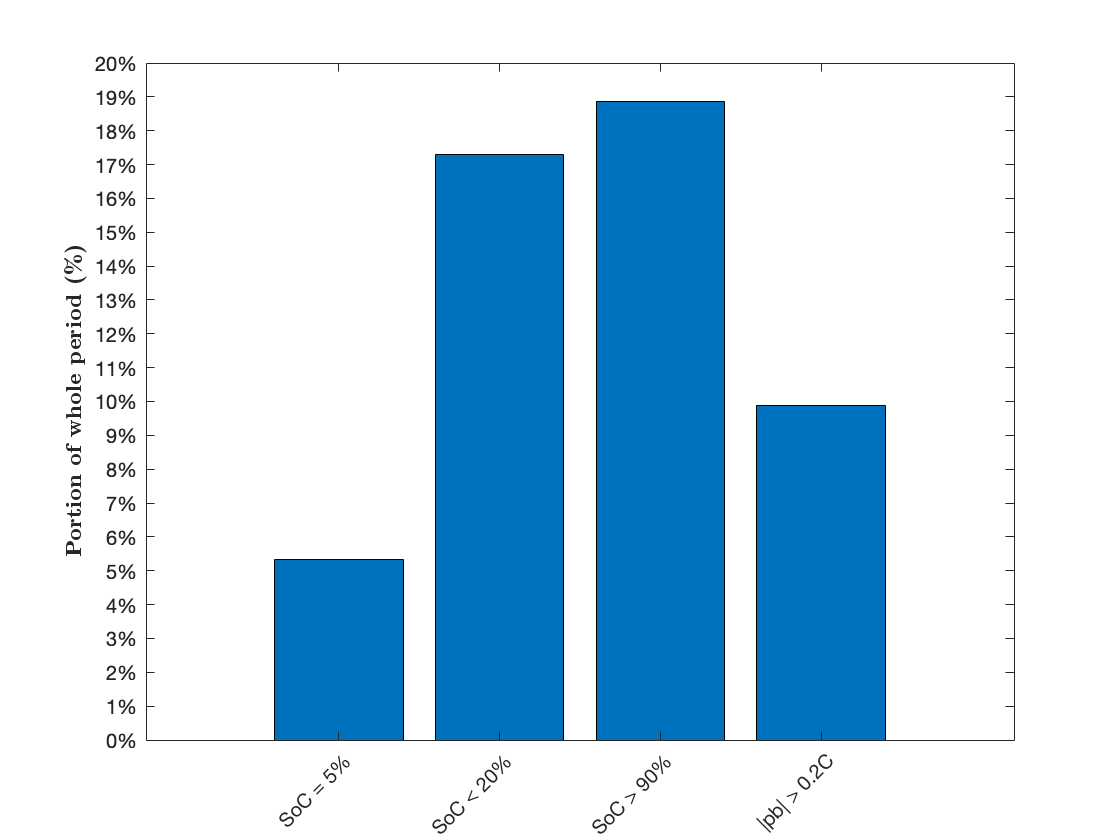
\includegraphics[width=\textwidth]{Figures/09Results/bANDpb02_231224-240101_CS_soiling26.png}
    \caption[Battery results current control system]{Number of times battery was in unhealthy states as a percentage of the whole period for the current control system. }
    \label{fig:bANDpb02_231224-240101_CS_soiling26}
\end{figure}


\begin{figure}[h]
    \centering
    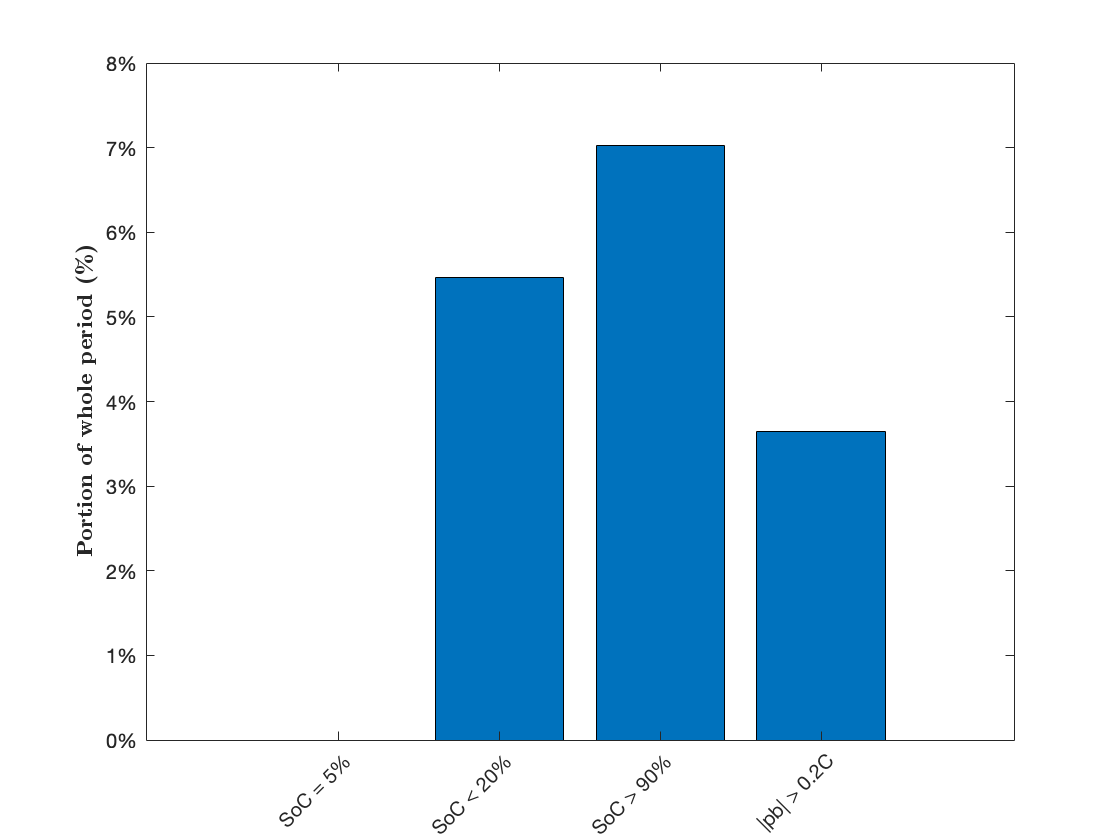
\includegraphics[width=\textwidth]{Figures/09Results/bANDpb02_231224-240101_tuning1_soiling26.png}
    \caption[Battery results proposed control system 1]{Number of times battery was in unhealthy states as a percentage of the whole period for the proposed control system with tuning 1. }
    \label{fig:bANDpb02_231224-240101_tuning1_soiling26}
\end{figure}

\begin{figure}[h]
    \centering
    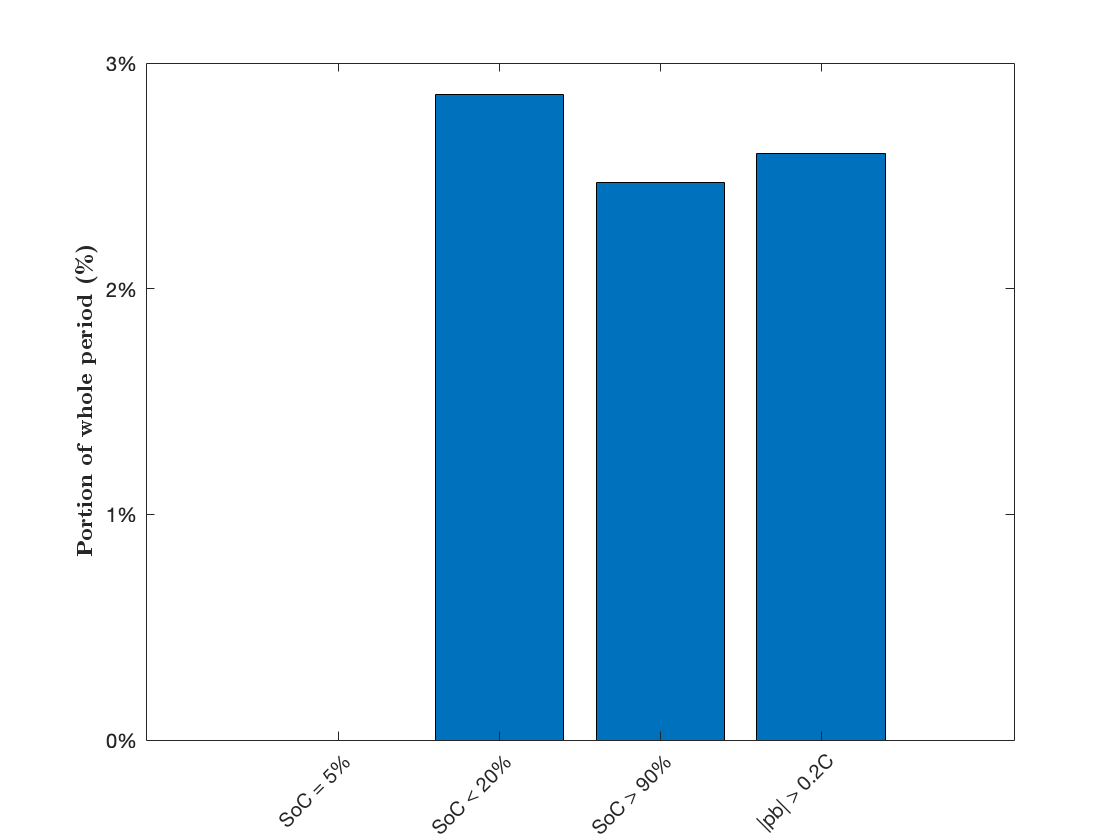
\includegraphics[width=\textwidth]{Figures/09Results/bANDpb02_231224-240101_tuning2_soiling26.png}
    \caption[Battery results proposed control system 2]{Number of times battery was in unhealthy states as a percentage of the whole period for the proposed control system with tuning 2. }
    \label{fig:bANDpb02_231224-240101_tuning2_soiling26}
\end{figure}

\begin{figure}[h]
    \centering
    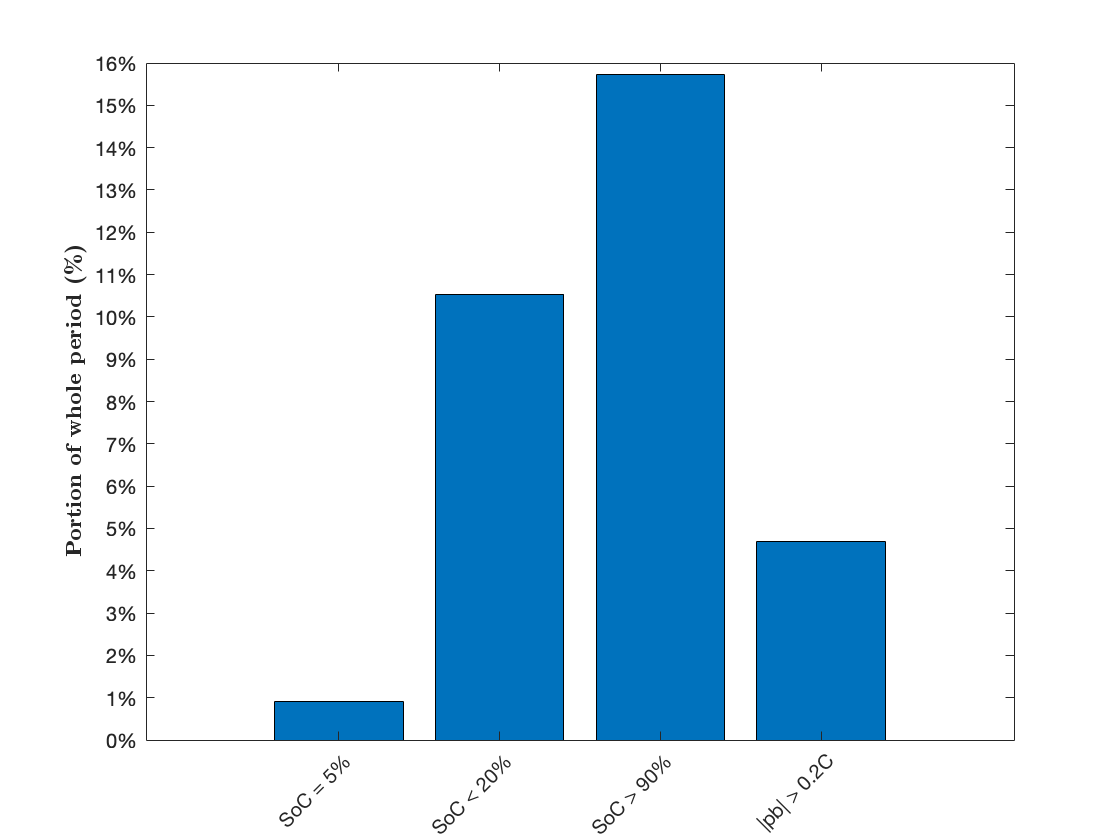
\includegraphics[width=\textwidth]{Figures/09Results/bANDpb02_231224-240101_tuning2_perfectR.png}
    \caption[Battery results proposed control system 2 perfect R]{Number of times battery was in unhealthy states as a percentage of the whole period for the proposed control system with tuning2 using perfect demand estimation. }
    \label{fig:bANDpb02_231224-240101_tuning2_perfectR}
\end{figure}

\subsection{Flexible Loads}

Flexible loads have a requested energy demand within the day. Figure \ref{fig:error_def_231224-240101_CS_soiling26}, \ref{fig:error_def_231224-240101_tuning1_soiling26} and \ref{fig:error_def_231224-240101_tuning1_soiling26} shows deviation from that demand. A positive value indicates an \textit{oversupply} meaning that more than the daily energy demand is supplied to the load, while a negative value indicates an \textit{undersupply} meaning that less than requested is supplied. Values at zero, as in figure \ref{fig:error_def_231224-240101_CS_soiling26} tell that the flexible load demand is matched exactly.

\begin{figure}[h]
    \centering
    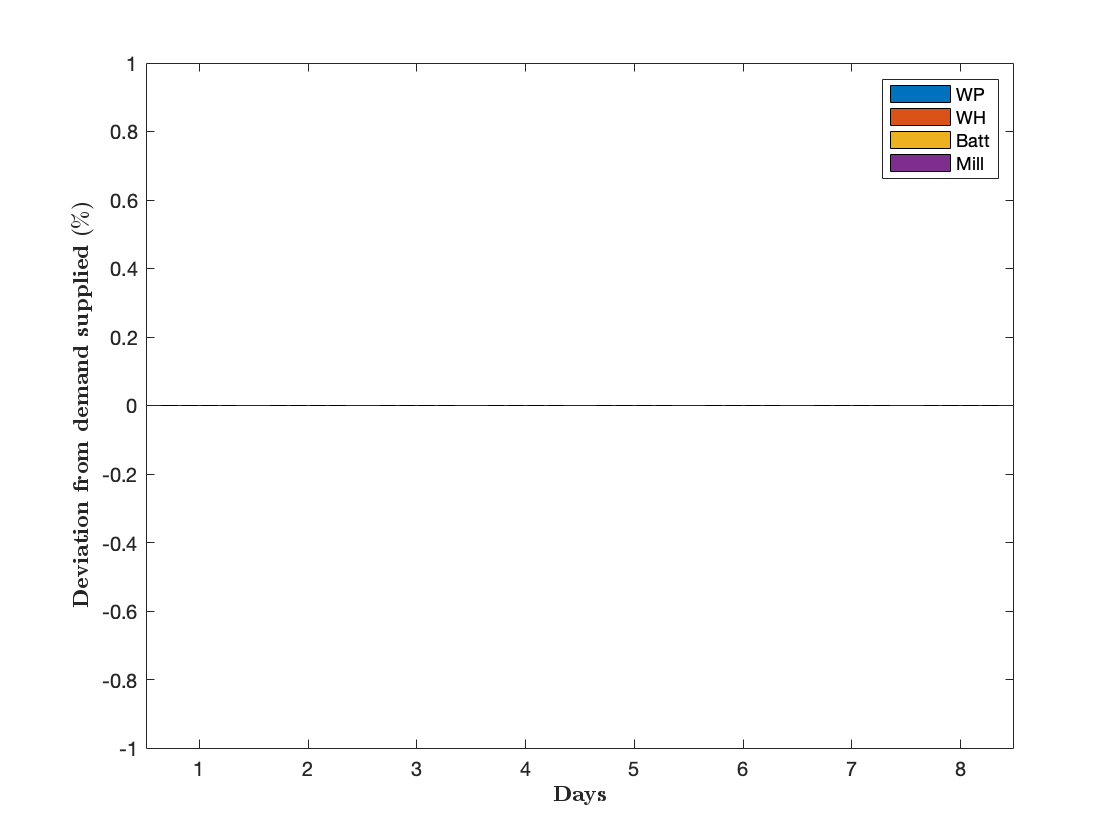
\includegraphics[width=\textwidth]{Figures/09Results/error_def_231224-240101_CS_soiling26.png}
    \caption[Flexible load deviation current control system]{The deviation from flexible load energy demand each day for the current control system. This plot indicates no deviation from flexible load demand by supply. }
    \label{fig:error_def_231224-240101_CS_soiling26}
\end{figure}

\begin{figure}[h]
    \centering
    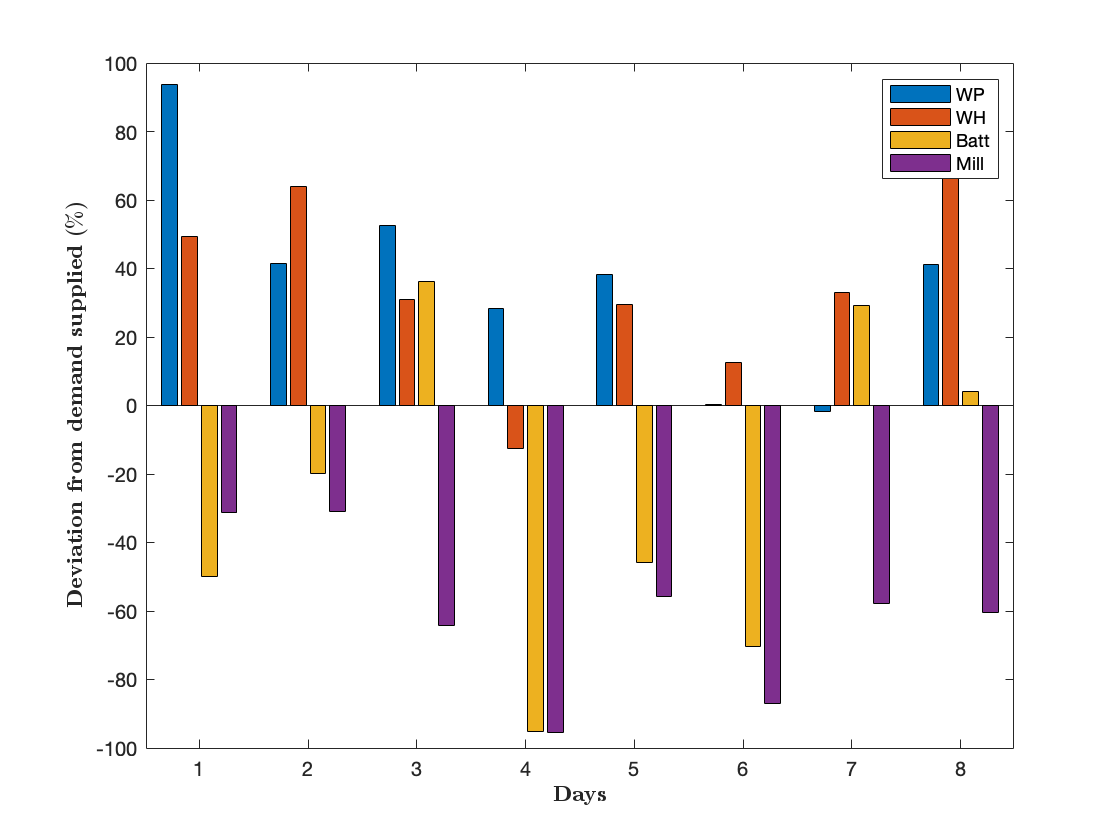
\includegraphics[width=\textwidth]{Figures/09Results/error_def_231224-240101_tuning1_soiling26.png}
    \caption[Flexible load deviation proposed control system 1]{The deviation from flexible load energy demand each day for the proposed control system with tuning 1. }
    \label{fig:error_def_231224-240101_tuning1_soiling26}
\end{figure}

\begin{figure}[h]
    \centering
    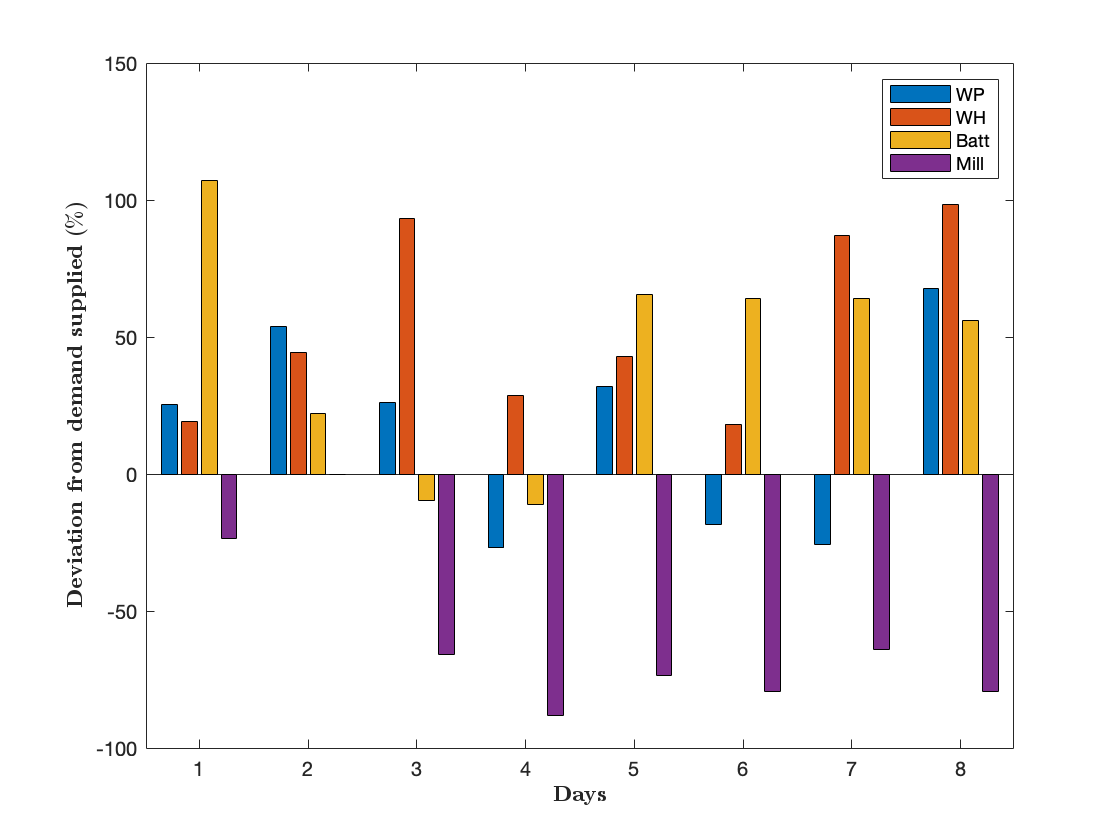
\includegraphics[width=\textwidth]{Figures/09Results/error_def_231224-240101_tuning2_soiling26.png}
    \caption[Flexible load deviation proposed control system 2]{The deviation from flexible load energy demand each day for the proposed control system with tuning 2. }
    \label{fig:error_def_231224-240101_tuning2_soiling26}
\end{figure}

\begin{figure}[h]
    \centering
    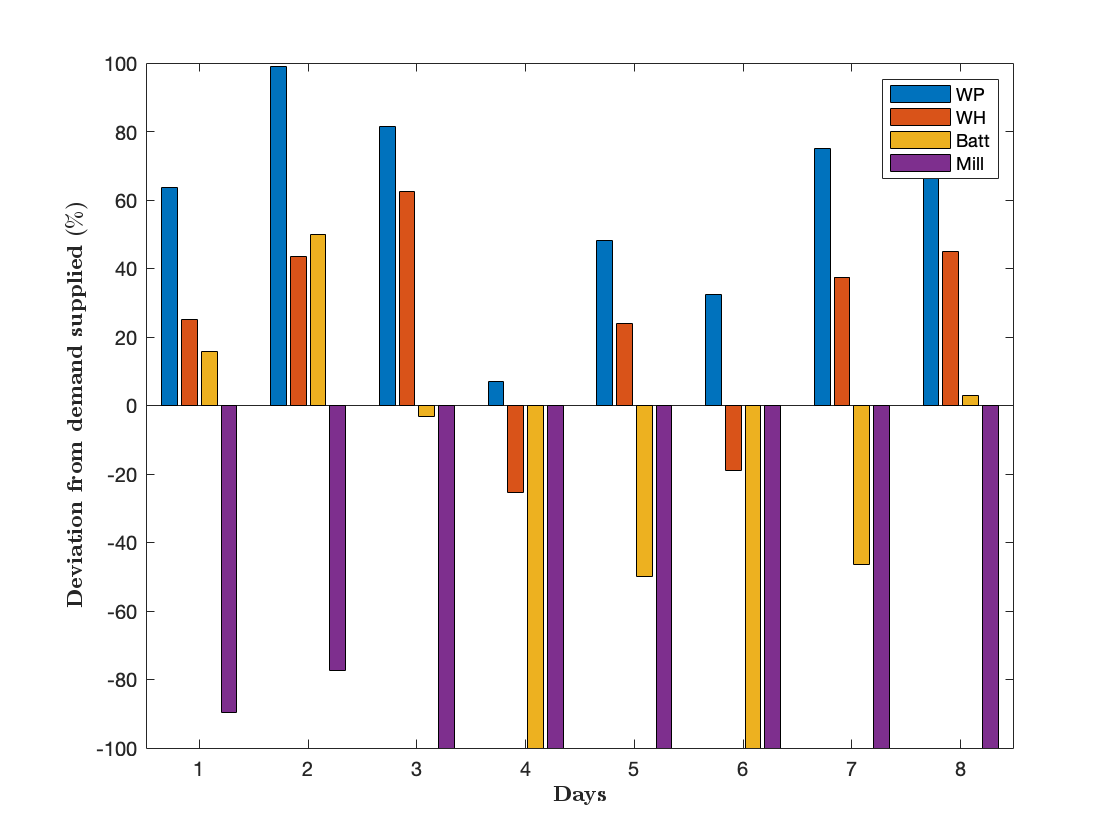
\includegraphics[width=\textwidth]{Figures/09Results/error_def_231224-240101_tuning2_perfectR.png}
    \caption[Flexible load deviation proposed control system 2 perfect R]{The deviation from flexible load energy demand each day for the proposed control system with tuning 2 using perfect demand estimation. }
    \label{fig:error_def_231224-240101_tuning2_perfectR}
\end{figure}

\subsection{Production}

Figure \ref{fig:prod_231224-240101_CS_soiling26}, \ref{fig:prod_231224-240101_tuning1_soiling26} and \ref{fig:prod_231224-240101_tuning2_soiling26} shows the relation between the potential and utilized production over time. 

\begin{figure}[h]
    \centering
    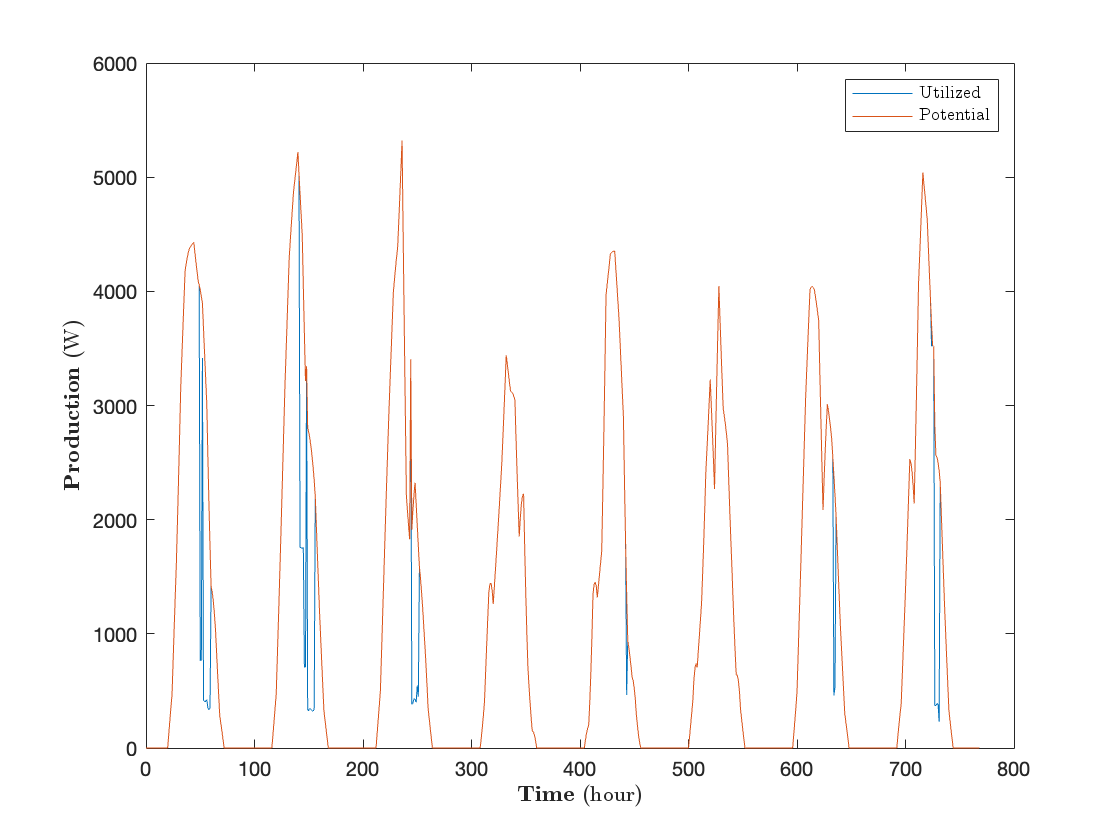
\includegraphics[width=\textwidth]{Figures/09Results/prod_231224-240101_CS_soiling26.png}
    \caption[Potential and utilized production current control system]{Potential and utilized production for each day for the current control system. }
    \label{fig:prod_231224-240101_CS_soiling26}
\end{figure}

\begin{figure}[h]
    \centering
    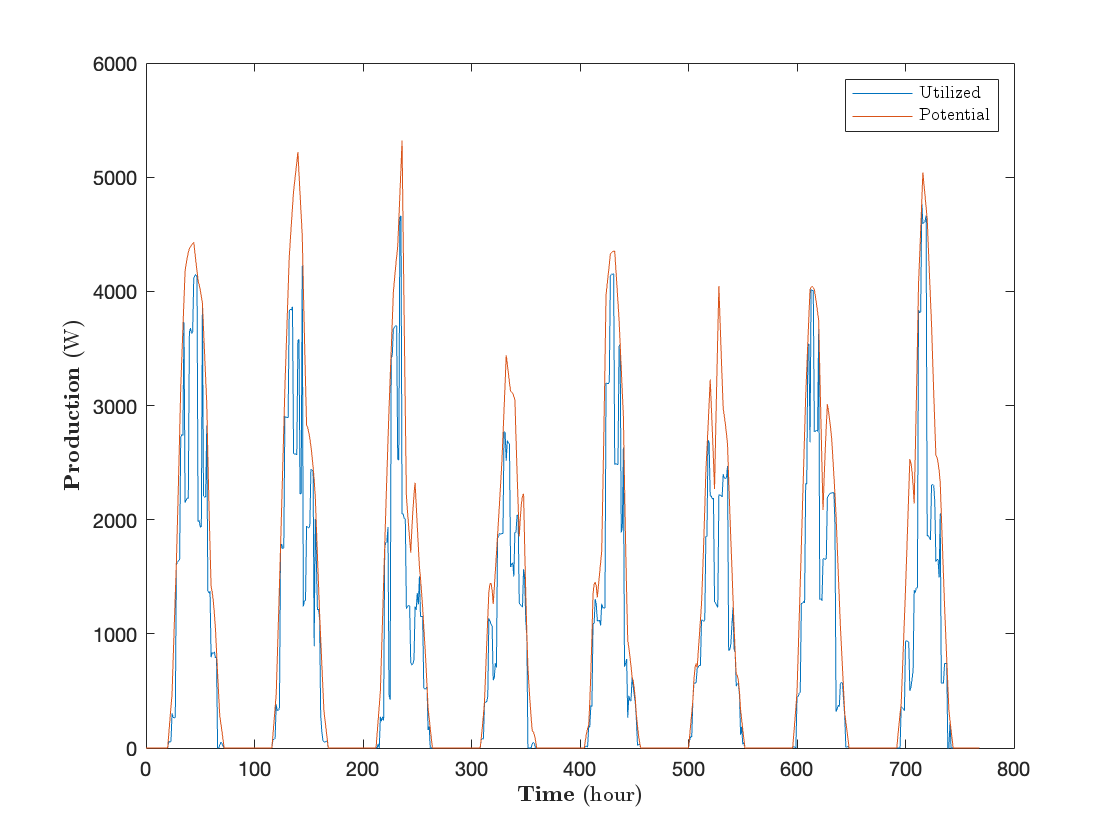
\includegraphics[width=\textwidth]{Figures/09Results/prod_231224-240101_tuning1_soiling26.png}
    \caption[Potential and utilized production proposed control system 1]{Potential and utilized production for each day for the proposed control system with tuning 1. }
    \label{fig:prod_231224-240101_tuning1_soiling26}
\end{figure}

\begin{figure}[h]
    \centering
    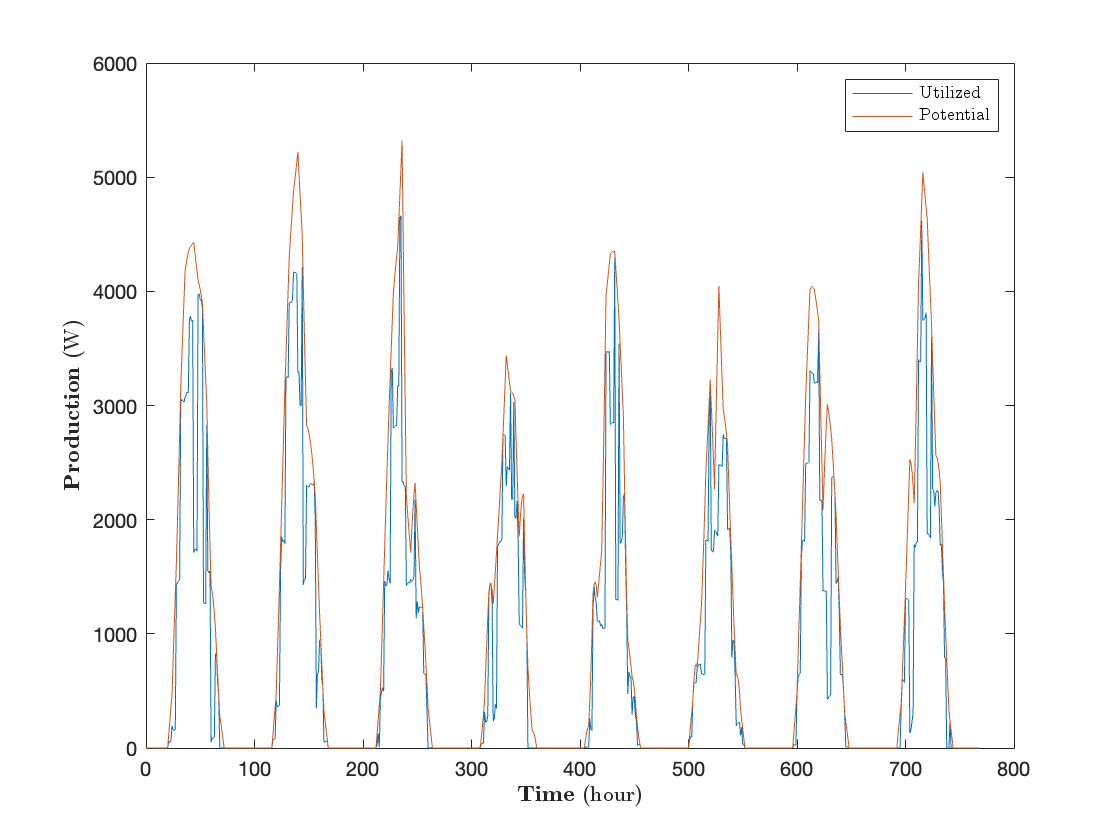
\includegraphics[width=\textwidth]{Figures/09Results/prod_231224-240101_tuning2_soiling26.png}
    \caption[Potential and utilized production proposed control system 2]{Potential and utilized production for each day for the proposed control system with tuning 2. }
    \label{fig:prod_231224-240101_tuning2_soiling26}
\end{figure}

\begin{figure}[h]
    \centering
    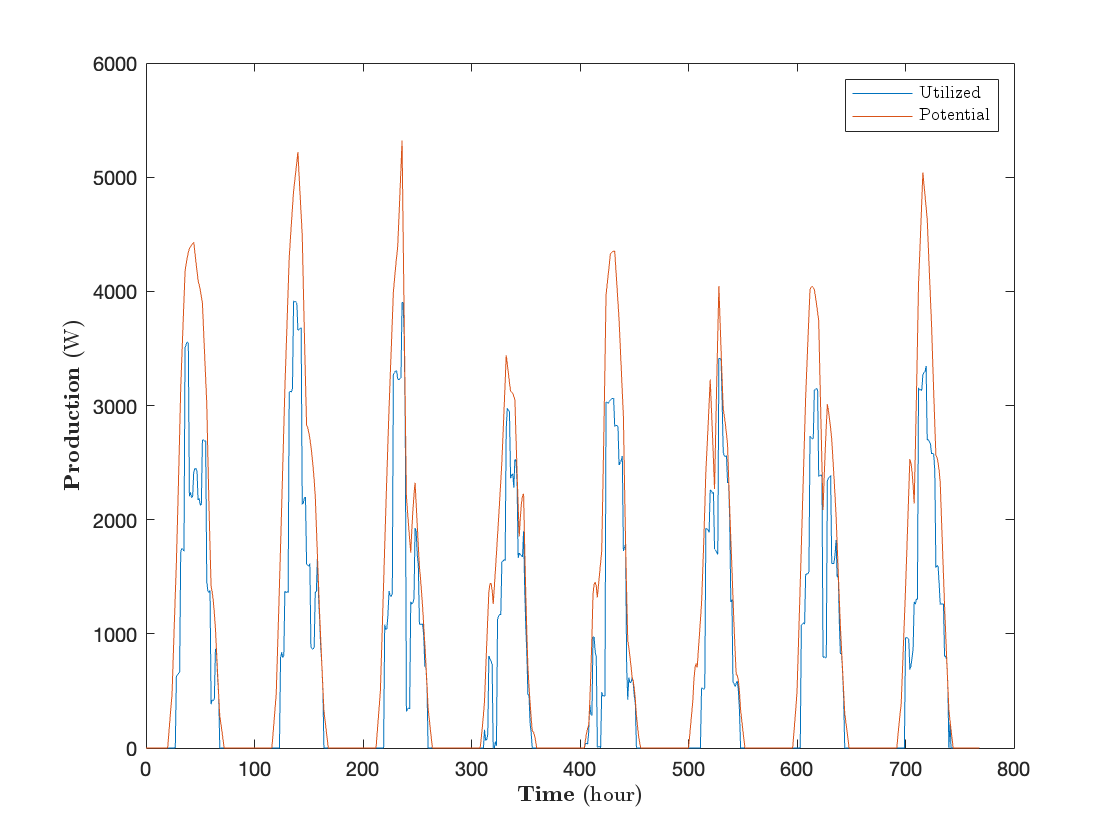
\includegraphics[width=\textwidth]{Figures/09Results/prod_231224-240101_tuning2_perfectR.png}
    \caption[Potential and utilized production proposed control system 2 perfect R]{Potential and utilized production for each day for the proposed control system with tuning 2 using perfect demand estimation. }
    \label{fig:prod_231224-240101_tuning2_perfectR}
\end{figure}


\subsection{Combined Results}
Table \ref{tab:combined_results_load} shows the combined results for the simulations concerning load and utilization. Table \ref{tab:combined_results_battery} shows the results concerning the battery health. The total load reliability expresses the reliability of combined reliability of all loads, while the critical expresses the reliability of medical loads. The reliability is measured using SAIDI from section \ref{sec:reliability}. 


\begin{table}[h]
    \centering
    \fontsize{12pt}{12pt}\selectfont
    \begin{tabular}{p{3cm}||p{2cm}|p{2.5cm}|p{2.5cm}|p{1cm}}
       Candidate  & Total reliability (\%) & Critical load reliability (\%) & Flexible Load Deviation (\%) & Utilization (\%)\\
       \hline
       \hline
       Current control system       & 96.86 & 97.14 & 0 & 91\\
       \hline
       Tuning1                      & 95.74 & 100 & -30.39 & 68\\
       \hline
       Tuning2                      & 95.84 & 99.80 & 112.24 & 70\\
       \hline
       Tuning2 perfect forecast     & 98.14 & 99.74 & -79.72 & 62\\
       
    \end{tabular}
    \caption[Simulation results - Load]{The combined simulation results relating to load.}
    \label{tab:combined_results_load}
\end{table}

\begin{table}[h]
    \centering
    \begin{tabular}{p{3cm}||p{2cm}|p{2cm}|p{2cm}|p{2cm}}
       Candidate  & b=5$\%$ (\%) &b<20$\%$ (\%) & b>90$\%$ (\%) & |pb|>0.2C$\%$ (\%)\\
       \hline
       \hline
        Current control system  & 5.33 & 17.30 & 18.86 & 9.88\\
       \hline
       Tuning1                  & 0 & 5.46 & 7.02 & 3.64\\
       \hline
       Tuning2                  & 0 & 2.86 & 2.47 & 2.60\\
       \hline
       Tuning2 perfect forecast & 0.91 & 10.53 & 15.73 & 4.68\\
       
    \end{tabular}
    \caption[Simulation results - Battery]{The combined simulation results relating to battery health. In the table, $b$ is the SOC while $pb$ is the charge/discharge-rate.}
    \label{tab:combined_results_battery}
\end{table}

\subsection{Critical Load Reliability at different battery capacities}
Figure \ref{fig:cr_reliability} shows the results regarding critical load reliability, for the current control system and proposed control system with tuning 2. The reliability is measured using SAIDI as described in section \ref{sec:reliability}. 

\begin{figure}[h]
    \centering
    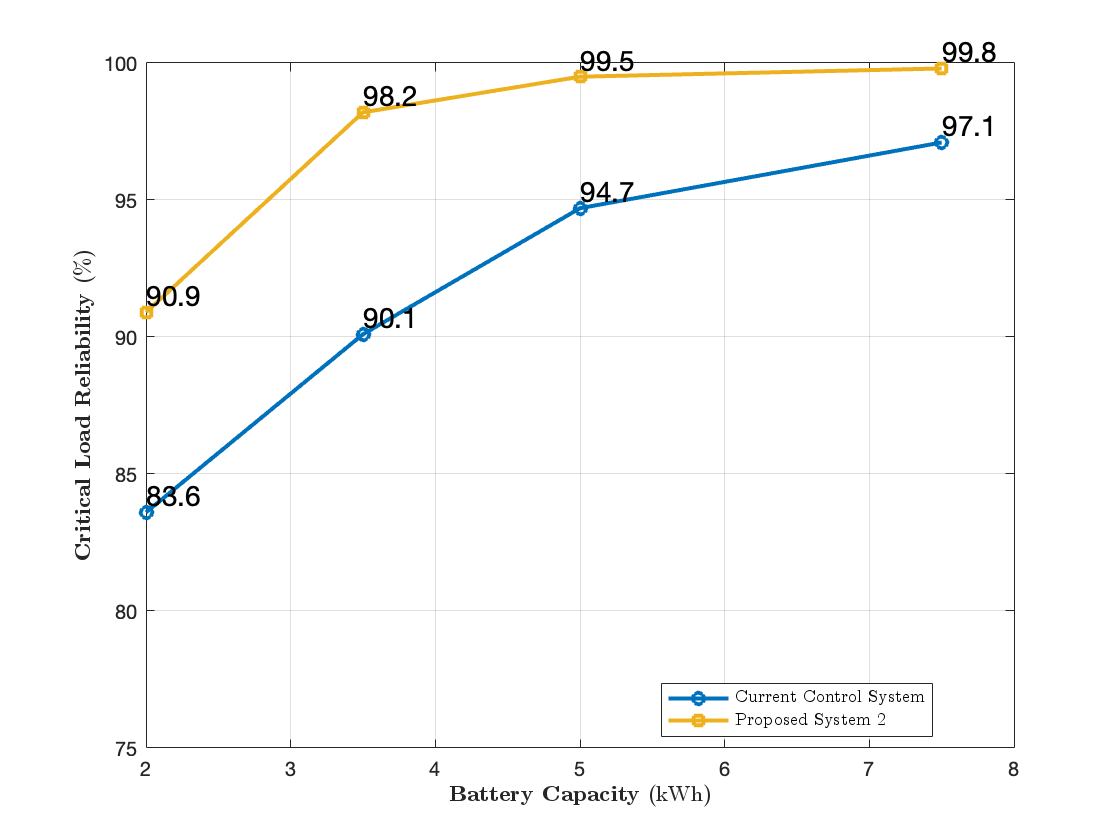
\includegraphics[width=\textwidth]{Figures/09Results/cr_reliability.png}
    \caption[Critical Load Reliability]{Critical load reliability at different battery capacities. Comparing the current control system (blue) and the proposed control system with tuning 2 (yellow). }
    \label{fig:cr_reliability}
\end{figure}